\documentclass[10pt, a4paper]{article}
\usepackage{amsmath}
\usepackage{amssymb}
\usepackage{mathtools}
\usepackage{mathtext}
\usepackage[T1, T2A]{fontenc}
\usepackage[utf8]{inputenc}
\usepackage[english, russian]{babel}
\usepackage{cmap}
\usepackage{fancyhdr}
\usepackage[pdftex]{graphicx}
\usepackage{gensymb}
\usepackage{floatrow}
\usepackage{titlesec}
\usepackage{lastpage}
\usepackage{float}
\usepackage{gensymb}
\usepackage{booktabs}
\usepackage{mathrsfs}
\usepackage{floatflt}
\usepackage{wrapfig}
\usepackage{caption}


\usepackage[figurename=Рис.]{caption}

\pagestyle{fancy}
	\fancyhf{}
	\lhead{\hspace{1bp} Работа \textnumero 4.4.2}
	\rhead{Терехов Максим 876\hspace{1bp}}
	\lfoot{Изучение фазовой решётки (эшелет)}
	\cfoot{\textbf{}}
	\rfoot{\thepage\ \textnormal{из}\ \pageref{LastPage}}
	\renewcommand{\headrulewidth}{1pt}
	\renewcommand{\footrulewidth}{1pt}


%\addtolength{\hoffset}{-1.75cm}
%\addtolength{\textwidth}{3.5cm} 

%\addtolength{\voffset}{-1.5cm}
%\addtolength{\textheight}{3cm} 

\titleformat{\section}
    [block]{\normalfont\bfseries\Large}{\rlap{\thesection}}{0em}
    {\vspace{-0.02\textwidth}\begin{minipage}[t]{.95\textwidth}}
[\end{minipage}]


\thispagestyle{fancy}

\captionsetup{justification=centering}



\begin{document}
\selectlanguage{russian}
\huge
\begin{center}
\textbf{Изучение фазовой решётки (эшелет)}
\end{center}
\parindent=1cm
\large
	\section*{Цель работы}
	
Знакомство с работой гониометра и определение спектральных характеристик фазовой решётки (эшелета).
	\section*{Оборудование}

	Ртутная лампа, гониометр, амплитудная и фазовая дифракционные решётки, плоскопараллельная стеклянная пластинка, призменный уголковый отражатель, щель с микрометрическим винтом.
\section*{Экспериментальная установка}
\begin{figure}[H]
	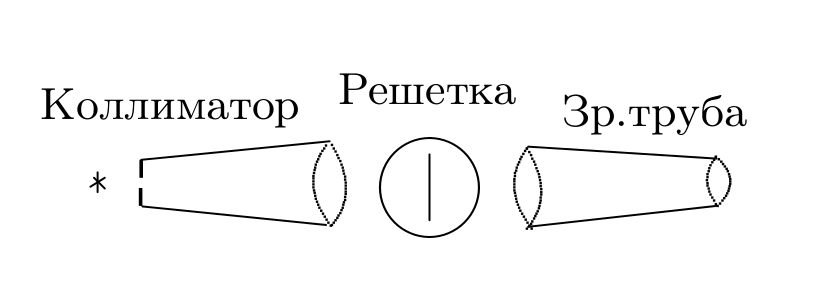
\includegraphics[width = 1.0\linewidth]{ust.png}
	\caption*{Схема экспериментальной установки (вид сверху)}
\end{figure}
\section*{Теоретическая часть}
Дифркационная решётка представляет собой стеклянную или металлическую пластину, на которую через строго одинаковые интервалы нанесены параллельные штрихи. Основные параметры дифракционной решётки "--- период $d$ (постоянная решётки), число штрихов $N$.
Условие дифракции Фраунгофера "--- решётка освещается плоской волной, а плоскость наблюдения практически находится в бесконечности.

 \begin{figure}[H]
	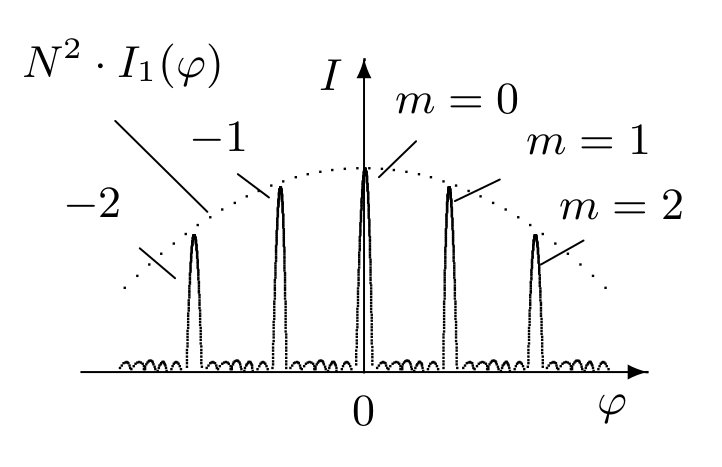
\includegraphics[width = 1.0\linewidth]{1.png}
	\caption*{Распределение интенсивности света при дифракции Фраунгофера на решётке}
\end{figure}

Согласно принципу Гюйгенса-Френеля распределение интенсивности в дифракционной картине определяется суперпозицией волн; амплитуды всех интерферирующих волн при $\varphi$ практически одинаковы; фазы составляют арифметическую прогрессию:
\[
	d \sin \varphi_m = m \lambda,
 \]
 где $m \in Z$ "--- порядок спектра.
 
 Интенсивность $I$ света, распространяющегося под углом $\varphi$ к нормали:
 \[
 I = I_1(\varphi)\frac{\sin^2 (N(dk \sin \varphi) / 2)}{\sin^2 ((dk \sin \varphi) 2)},
 \]
 где $k = \frac{2 \pi}{\lambda}$ "--- волновое число.
 
 Дисперсия $D$ характеризует угловое расстояние между близкими спектральными линиями:
 \[
 D = \frac{d \varphi}{d \lambda} = \frac{m}{d \cos \varphi} = \frac{m}{\sqrt{d^2 - m^2 \lambda^2}}
 \]
 Согласно притерию разрешения Релея, линии становятся неразличимыми, когда расстояние между ними меньше, чем растояние от максимума одной линии до её первого минимума:
 \[
 	\frac{Nkd}{2}(\sin (\varphi + \Delta \varphi) - \sin \varphi) = \pi,
 \]
 где $\Delta \varphi$ "--- угловая полуширина главного максимума, $\Delta \varphi = \frac{\lambda}{Nd \cos \varphi}$
 
 
 Разрешающая способность спектрального прибора $R$ вычисляется по формуле:
 \[
 R = \frac{\lambda}{\Delta \lambda} = m \cdot N
 \]
 \begin{figure}[H]
	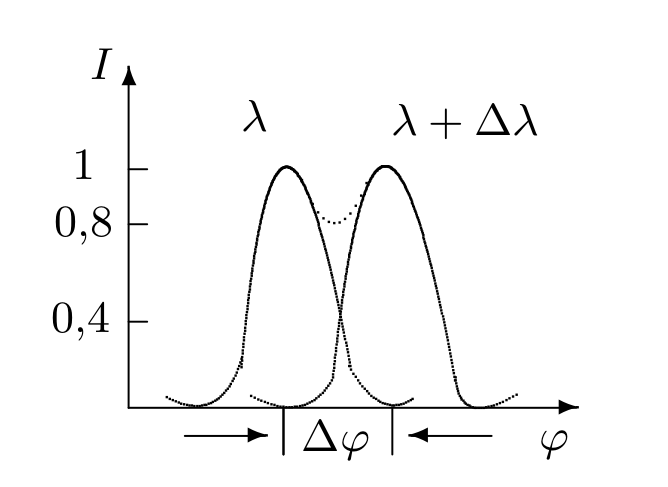
\includegraphics[width = 1.0\linewidth]{k.png}
	\caption*{К определению разрешающей способности дифракционной решётки}
\end{figure}
Дисперсионная область $G$ "--- предельная ширина спектрального интервала $d \lambda$, при которой спектры соседних порядков перекрываются только своими границами:
\[
G = d \lambda = \frac{\lambda}{m}.
\]
\section*{Обработка результатов экспериментов}
При работе с дифракционной решёткой основной задачей является точное измерение углов, при которых наблюдается главные максимум для различных длин волн.
Эшелет "--- отражательная решётка с  треугольным профилем штриха, в которой угол $\Omega$ между рабочей гранью и плоскостью решётки не превышает $20^o$
Рабочий порядок $m \leq 10$, число штрихов $n = 1200\ штр/мм$.

Угол, под которым наблюдается максимум интенсивности функции $I_1 (\varphi)$, соответствует зеркальному отражению падающего луча от грани и называется углом блеска $\varphi_б$.
\[
	\varphi_б = \psi + 2 \Omega,
\]
где $\psi$ "--- угол, под которым падает плоская монохроматическая волна $\lambda$.

Разность хода $\Delta$ кратна $\lambda$:
\[
\Delta = d (\sin \varphi_m - \sin \varphi) = m \lambda.
\]
Изменяя угол падения, можно добиться того, чтобы угол блеска совпал с углом дифракции спектра одного из порядков; в этом порядке спектр будет наиболее ярким. Этот порядок принять называть рабочим.
\begin{figure}[H]
	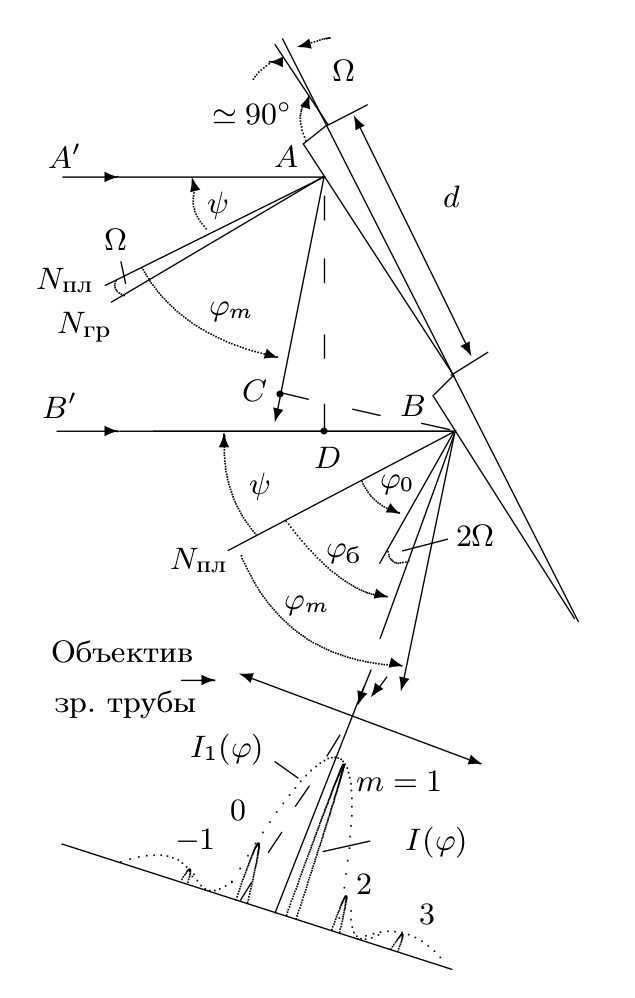
\includegraphics[width = 0.5\linewidth]{3.png}
	\caption*{Распределение интенсивности в спектре эшелета}
\end{figure}

Чтобы устранить произвол в выборе угла падения, принято считать, что решётка должна работать в автоколлиматорном режиме. В этом случае условие $d(\sin \\varphi_m + \sin \varphi) = m \lambda$ принимает вид:
\[
	2d \sin \Omega = m_p \lambda_p.
\]
Для оценки $\Delta \varphi_m$ воспользуемся методом векторных диаграмм:
\begin{figure}[H]
	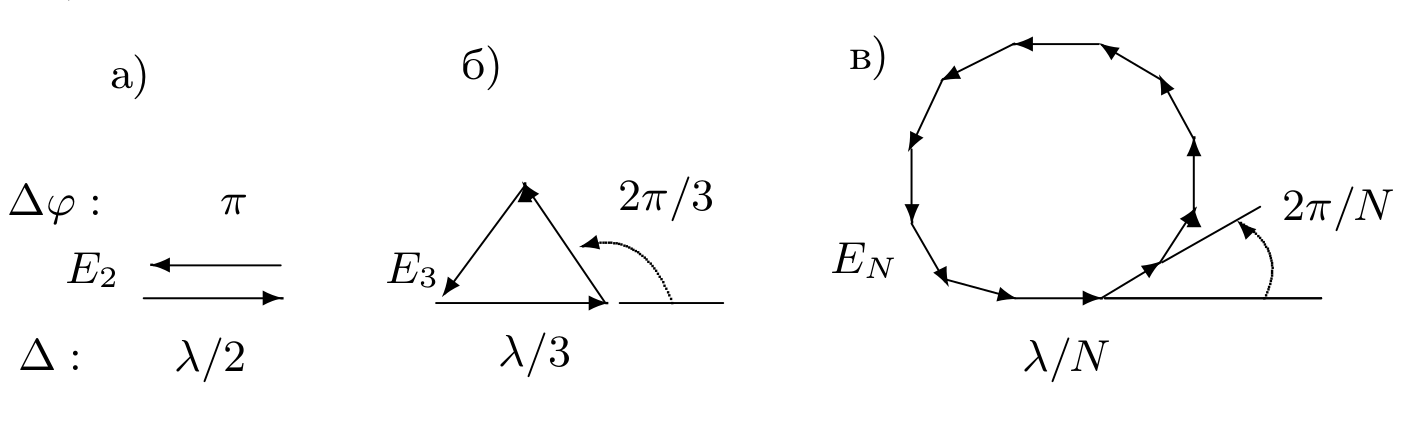
\includegraphics[width = 1.0\linewidth]{2.png}
	\caption*{Векторные диаграммы}
\end{figure}
Направление на минимум, ближайший к максимуму любого порядка:
\[
d(\sin(\varphi_m + \Delta \varphi) + \sin \psi) = m \lambda + \frac{\lambda}{N}
\]
Для малой полуширины максимума получим:
\[
\Delta \varphi = \frac{\lambda}{Nd\cos \phi_m}
\]
Зависимость дисперсии $D$ от параметров эшелета:
\[
D = \frac{m}{d \cos \varphi_m} = \frac{m}{\sqrt{d^2 - (m \lambda - d \sin \psi)^2}}
\]

\section*{Результаты и обработка}
Произведём юстировку гониометра и установим начало отсчёта, руководствуясь техническим описанием.11321

Держа эшлет в вытянутой руке, найдём отражение лампы накаливанияж вращая эшелет вокруг оси, рассмотрим спектры положительных и отрицательных порядков; определим рабочий порядок; оценим дисперсионную область и сравним её с шириной спектра лампы:

\noindent
Средние значения:
\[
	\lambda = 600\ нм; \quad \Delta \phi = 200\ нм;
\]
\[
	G = \frac{\lambda}{m} = 200\ нм; \quad \text{Рабочий порядок}\ m_p = -1.
\]
Проделаем дополнительную настройку столика с эшелетом; установим $\psi = 30^o$; подберём ширину входной щели так, чтобы хорошо разрешались линии жёлтого дублета (ширина изображения щели чуть больше промежутка между линиями двойного штриха); установим высоту щели, удобную для измерений.

Для угла $\psi = 45^o$ измерим угловые координаты спектральных линий ртути в рабочем порядке. Отметим гловую координату каждой из описанных линий:
\begin{table}[H]
\centering
\begin{tabular}{|c|c|c|}  \hline
Ахроматический & $93^o 10' 30''$ & {} \\\hline
Фиолетовый & $75^o 36' 45''$ & $4047 \dot A$ \\\hline
Синий & $74^o 23' 45''$ & $4358 \dot A$ \\\hline
Голубой & $72^o15'35''$ & $4916 \dot A$ \\\hline
	Зелёный & $70^o12'35''$ & $5461 \dot A$ \\\hline
Желтый 2 & $69^o 3' 25''$ & $5770 \dot A$ \\\hline
Жёлтый 1 & $68^o 58'35''$ & $5791 \dot A$ \\\hline
\end{tabular}
\end{table}
Для оценки разрешающей способности измерим гирину одной из линий жёлтого дублета и рассчитаем аппаратную полуширину линии $\Delta \lambda$:
\[
\text{Ширина линии:}\ 68^o2'10'' - 68^o2'0'' = 10'' 
\]
\[
\Delta \lambda = \frac{1}{3} \dot A; \quad R = \frac{\lambda}{\Delta \lambda} =\frac{5770}{20} \cdot 60 =  17810
\]
Для угла $\psi = 30^o$ измерим координаты каждой из жёлтых линий во всех наблюдаемых порядках:
\begin{table}[H]
\begin{center}
\begin{tabular}{|c|c|c|} \hline
& $Ж_1$ & $89^o3'55''$ \\
\cline{2-3}
$I_{пол}$
& $Ж_2$ & $88^055'45''$ \\\hline
& $Ж_1$ & $39^o50'55''$ \\
\cline{2-3}
$I_{отр}$
& $Ж_2$ & $39^o55'25''$ \\\hline
\end{tabular}
\end{center}
\end{table}
Повторим измерения для $\psi = 45^0, 60^o$:

\begin{table}[H]	
\begin{center}
\begin{tabular}{|c|c|c|} \hline
& $Ж_1$ & $68^058'35''$\\
\cline{2-3}
$I_{отр}$
& $Ж_2$ & $69^o3'35''$ \\\hline
& $Ж_1$ & $48^o32'15''$ \\
\cline{2-3}
$II_{отр}$
& $Ж_2$ & $48^o40'50''$ \\\hline
\end{tabular}
\caption{$\psi = 45^o$}
\end{center}
\end{table}

\begin{table}[H]	
\begin{center}
\begin{tabular}{|c|c|c|} \hline
& $Ж_1$ & $92^o15'5''$\\
\cline{2-3}
$I_{отр}$
& $Ж_2$ & $92^o20'15''$ \\\hline
& $Ж_1$ & $70^o51'45''$ \\
\cline{2-3}
$II_{отр}$
& $Ж_2$ & $71^o0'35''$ \\\hline
& $Ж_1$ & $50^o51'5''$\\
\cline{2-3}
$III_{отр}$
& $Ж_2$ & $51^o4'45''$ \\\hline
\end{tabular}
\caption{$\psi = 60^o$}
\end{center}
\end{table}
\textbf{Зависимость разрешающей силы от ширины пучка:}

Натроим зрительную трубу на желтый дублет в рабочем порядке; определим начало отсчёта "--- момент открытия щели. Крест появляется при $59^o57'20''$; ширина щели "--- 3 деления.

Откроем щель пошире; уменьшая ширину щели, добьемся предельного разрешения желтого дублета, оценим число штрихов:
\[
	 n \approx 1600\ штр/мм; \quad \Delta \lambda = 2 \dot A.
\]
Построим график зависимости $\sin \varphi_m = f(\lambda)$ и по углу наклона определим период эшелета:
\begin{figure}[H]
	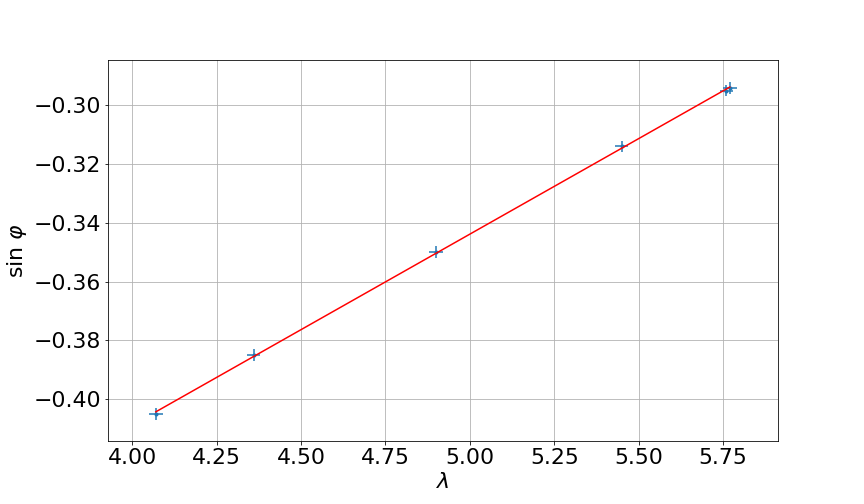
\includegraphics[width = 1.0\linewidth]{g1.png}
	\caption*{Зависимость $\sin \varphi_m$ от $\lambda$}
\end{figure}
Угол наклона графика $k = (6.5 \pm 0.1)\cdot 10^6$

Число штрихов $n \approx 650 \pm 10\ штр/мм$

Период эшелета: $d = \frac{1}{0.65} = 1.53 \pm 0.04$ мм.

Угловая дисперсия в рабочем порядке для жёлтого дублета в угловых секундах на $\dot A$:
\[
D = 14.3\ \frac{угл \cdot сек}{\dot A}
\]
Экспериментальная разрешающая способность:
\[
R = \frac{\lambda}{\Delta \lambda} = 2890
\]
\newpage
\section*{Вывод}
В данной лабораторной работе мы исследовали спектральные характеристики дифракционной решётки, научились работать с гониометром, экспериментально определили период решётки и  разрешающую способность.
\end{document}
